\chapter{Modello delle incertezze}
\section{Obiettivo e principio di modellazione}
Il modello incerto deve mantenere i fenomeni fisici rilevanti senza rendere opaca la struttura $\Delta$. Definiamo quindi un solo insieme di progetto. Non esistono scenari gerarchici: ogni percentuale è un'ipotesi ingegneristica, non una tolleranza misurata o un intervallo di confidenza.

\section{Parametri reali \texttt{ureal}}
Le due rigidezze SEA sono incluse perché modificano direttamente coppia elastica e modi flessibili; $J_{m1}$ rappresenta l'incertezza sull'inerzia riflessa del primo azionamento. Tutti e tre i parametri usano la variazione semplice $\pm10\%$:
\begin{verbatim}
k1  = ureal('k1',  p.Ks(1,1), 'Percentage', 10);
k2  = ureal('k2',  p.Ks(2,2), 'Percentage', 10);
Jm1 = ureal('Jm1', p.Jm(1,1), 'Percentage', 10);
\end{verbatim}
Ogni oggetto è riutilizzato in tutte le occorrenze delle equazioni e resta un singolo blocco reale scalare. Gli altri parametri sono nominali per mantenere l'ensemble leggibile; ciò non equivale a dichiararli fisicamente certi.

La scelta di $k_1$ e $k_2$ è legata alla natura SEA: una variazione di rigidezza cambia sia la coppia elastica $K_s(\theta-q)$ sia la posizione dei modi flessibili. $J_{m1}$ rappresenta invece una direzione di incertezza inerziale del drive train. Il valore $\pm10\%$ è un inviluppo ingegneristico semplice, adottato in assenza di dati di identificazione; non è ricavato da una distribuzione statistica. Per evitare di moltiplicare blocchi scarsamente giustificati, $m_1,m_2,l_1,l_2,J_{m2},B_{m1},B_{m2}$ e $g$ restano nominali. Le masse e le geometrie definiscono il modello rigido adottato, $J_{m2}$ non duplica la direzione già rappresentata da $J_{m1}$, gli smorzamenti sono termini dissipativi piccoli e $g$ è una costante ambientale. Questa esclusione è una scelta di modello, non una dichiarazione di certezza fisica.

Un parametro \texttt{ureal} conserva una dipendenza reale e ripetuta: se $k_1$ compare in più elementi di $A$, tutte le occorrenze variano in modo coerente attraverso lo stesso scalare normalizzato. È quindi adatto a una dispersione parametrica strutturata. Un blocco \texttt{ultidyn}, usato più avanti per $W_I\Delta$, descrive invece una dinamica stabile non nota entro un limite in norma; non possiede un unico valore fisico come rigidezza, massa o ritardo.


\medskip\noindent\textbf{Derivazione manuale della LFT meccanica.}
Affianchiamo alla costruzione automatica una rappresentazione ottenuta dalle
equazioni SEA, senza cambiarne equilibrio o parametri. Poniamo
$x=[q^\top,\dot q^\top,\theta^\top,\dot\theta^\top]^\top$,
$t=[\tau^\top,d^\top]^\top$, $K_r=0.1K_{s0}$ e
$j_r=0.1J_{m1,0}e_1$. La coppia elastica incerta è
$K_{s0}(\theta-q)+K_r w_k$, con
$w_k=\operatorname{diag}(\delta_{k1},\delta_{k2})(\theta-q)$.
L'equazione motore si scrive esattamente come
\[
 J_{m0}\ddot\theta=\tau-B_m\dot\theta-K_{s0}(\theta-q)
                   -K_r w_k-j_r w_J,\qquad
 w_J=\delta_J\ddot\theta_1.
\]
Questa chiusura conserva l'inverso dell'inerzia: non sostituisce
$1/J_{m1}$ con una linearizzazione. Con $M_\ell$ matrice d'inerzia
link all'equilibrio e $(A_0,B_0,C_0)$ della meccanica nominale,
\[
 B_w=\begin{bmatrix}
 0_{2\times3}\\ M_\ell^{-1}[K_r\ \ 0]\\0_{2\times3}\\
 -J_{m0}^{-1}[K_r\ \ j_r]
 \end{bmatrix},\qquad
 \dot x=A_0x+B_0t+B_ww_\Delta.
\]
Le porte verso l'incertezza sono
$v_\Delta=[(\theta-q)^\top,\ddot\theta_1]^\top$.
Se $e_7$ seleziona la prima accelerazione motore in $\dot x$,
\[
 C_v=\begin{bmatrix}[-I\  0\  I\  0]\\e_7^\top A_0\end{bmatrix},
 \quad D_{vw}=\begin{bmatrix}0_{2\times3}\\e_7^\top B_w\end{bmatrix},
 \quad D_{vt}=\begin{bmatrix}0_{2\times4}\\e_7^\top B_0\end{bmatrix}.
\]
La parte nota $M_m$ ha realizzazione
$(A_0,[B_w\ B_0],[C_v;C_0], [D_{vw}\ D_{vt};0_{2\times7}])$,
cinque uscite $[v_\Delta;q]$ e sette ingressi $[w_\Delta;t]$.
Il blocco $\Delta_m=\operatorname{diag}(\delta_{k1},\delta_{k2},\delta_J)$
è $3\times3$ e ciascuno scalare appartiene a $[-1,1]$.
La chiusura è ben posta perché $1+0.1\delta_J\ge0.9$.
Nel codice \texttt{lft(Delta,M)} richiude queste prime porte; la
costruzione non usa \texttt{lftdata} per ottenere le matrici manuali.
\begin{center}
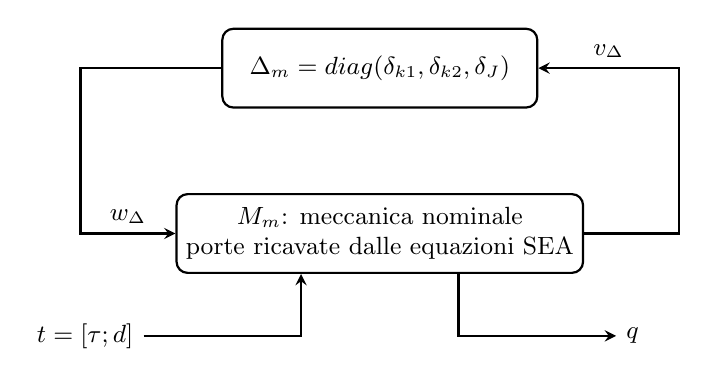
\begin{tikzpicture}[>=stealth,thick,every node/.style={font=\small},
 b/.style={draw,rounded corners,align=center,minimum width=4cm,minimum height=1cm}]
\node[b] (m) at (0,0) {$M_m$: meccanica nominale\\porte ricavate dalle equazioni SEA};
\node[b] (d) at (0,2.1) {$\Delta_m=\operatorname{diag}(\delta_{k1},\delta_{k2},\delta_J)$};
\draw[->] (m.east) -- (3.8,0) -- (3.8,2.1) -- node[above] {$v_\Delta$} (d.east);
\draw[->] (d.west) -- (-3.8,2.1) -- (-3.8,0) -- node[above] {$w_\Delta$} (m.west);
\draw[->] (-3,-1.3) node[left] {$t=[\tau;d]$} -- (-1,-1.3) -- (m.south -| -1,0);
\draw[->] (m.south -| 1,0) -- (1,-1.3) -- (3,-1.3) node[right] {$q$};
\end{tikzpicture}

\end{center}
Il confronto con la meccanica automatica usa il nominale, tutti gli otto
vertici e 24 punti interni con seed 20261026. Su 1601 frequenze fra
$10^{-4}$ e $10^5$ rad/s lo scarto relativo massimo è
$1.71\cdot10^{-14}$. La derivazione stabilisce l'identità strutturale;
i campioni ne controllano l'implementazione numerica.

\section{Incertezza dinamica degli attuatori}
Per ciascun drive assumiamo $\omega_n$ e $\zeta$ in $\pm10\%$ e il ritardo in $\pm20\%$. Il ritardo ha un intervallo più ampio perché include latenza e jitter. La famiglia di verifica contiene il nominale con ritardo esatto, sei variazioni singole, otto corner e 105 campioni riproducibili.

La convenzione input-moltiplicativa è
\[
G_{a,i}(s)=G_{a,0}(s)[1+W_I(s)\Delta_i(s)],\qquad
\|\Delta_i\|_\infty\le1.
\]
La forma dell'inviluppo presenta una sola transizione principale; viene perciò scelto un peso di ordine uno e \texttt{ucover} ne calcola i coefficienti. Non viene eseguito un ranking di ordini. Il peso finale è stabile e proprio; la copertura è verificata sui campioni e sulle frequenze della griglia, con safety factor 1.08 e rapporto massimo $|E|/|W_I|=0.92593$.

Il range $\pm10\%$ su $\omega_n$ e $\zeta$ rappresenta la variazione moderata della banda e dello smorzamento al mutare di drive e carico. Sul ritardo si usa $\pm20\%$: la latenza nominale di 15 ms può includere non soltanto dispersioni parametriche, ma anche scheduling e jitter, per i quali un inviluppo relativo più ampio è prudente. Questi tre parametri servono a costruire la famiglia di errori; nella pianta incerta finale la famiglia è condensata nel canale dinamico $W_I\Delta$, evitando di trattare un ritardo come un semplice scalare reale.

I due canali usano $\Delta_{act1}$ e $\Delta_{act2}$ indipendenti. Un unico blocco avrebbe imposto una correlazione perfetta non supportata da dati. La struttura finale è:
% Generated by build_m18_report_tables.m. Do not edit.
\begin{table}[H]
\centering
\resizebox{\textwidth}{!}{%
\begin{tabular}{llll}
\toprule
Parametro & Nominale & Range & Rappresentazione \\
\midrule
k2 & 40 & 7\% & parametrica reale \\
k1 & 50 & 7\% & parametrica reale \\
Jm1 & 0.01 & 9\% & parametrica reale \\
wn & 40 & 8\% & famiglia coperta da $W_I\Delta$ \\
zeta & 0.8 & 7.5\% & famiglia coperta da $W_I\Delta$ \\
delay & 0.015 & 20\% & famiglia coperta da $W_I\Delta$ \\
\bottomrule
\end{tabular}
}
\caption{Incertezze ingegneristiche M4; i range non sono distribuzioni probabilistiche identificate.}
\label{tab:uncertainties}
\end{table}


\begin{figure}[H]\centering
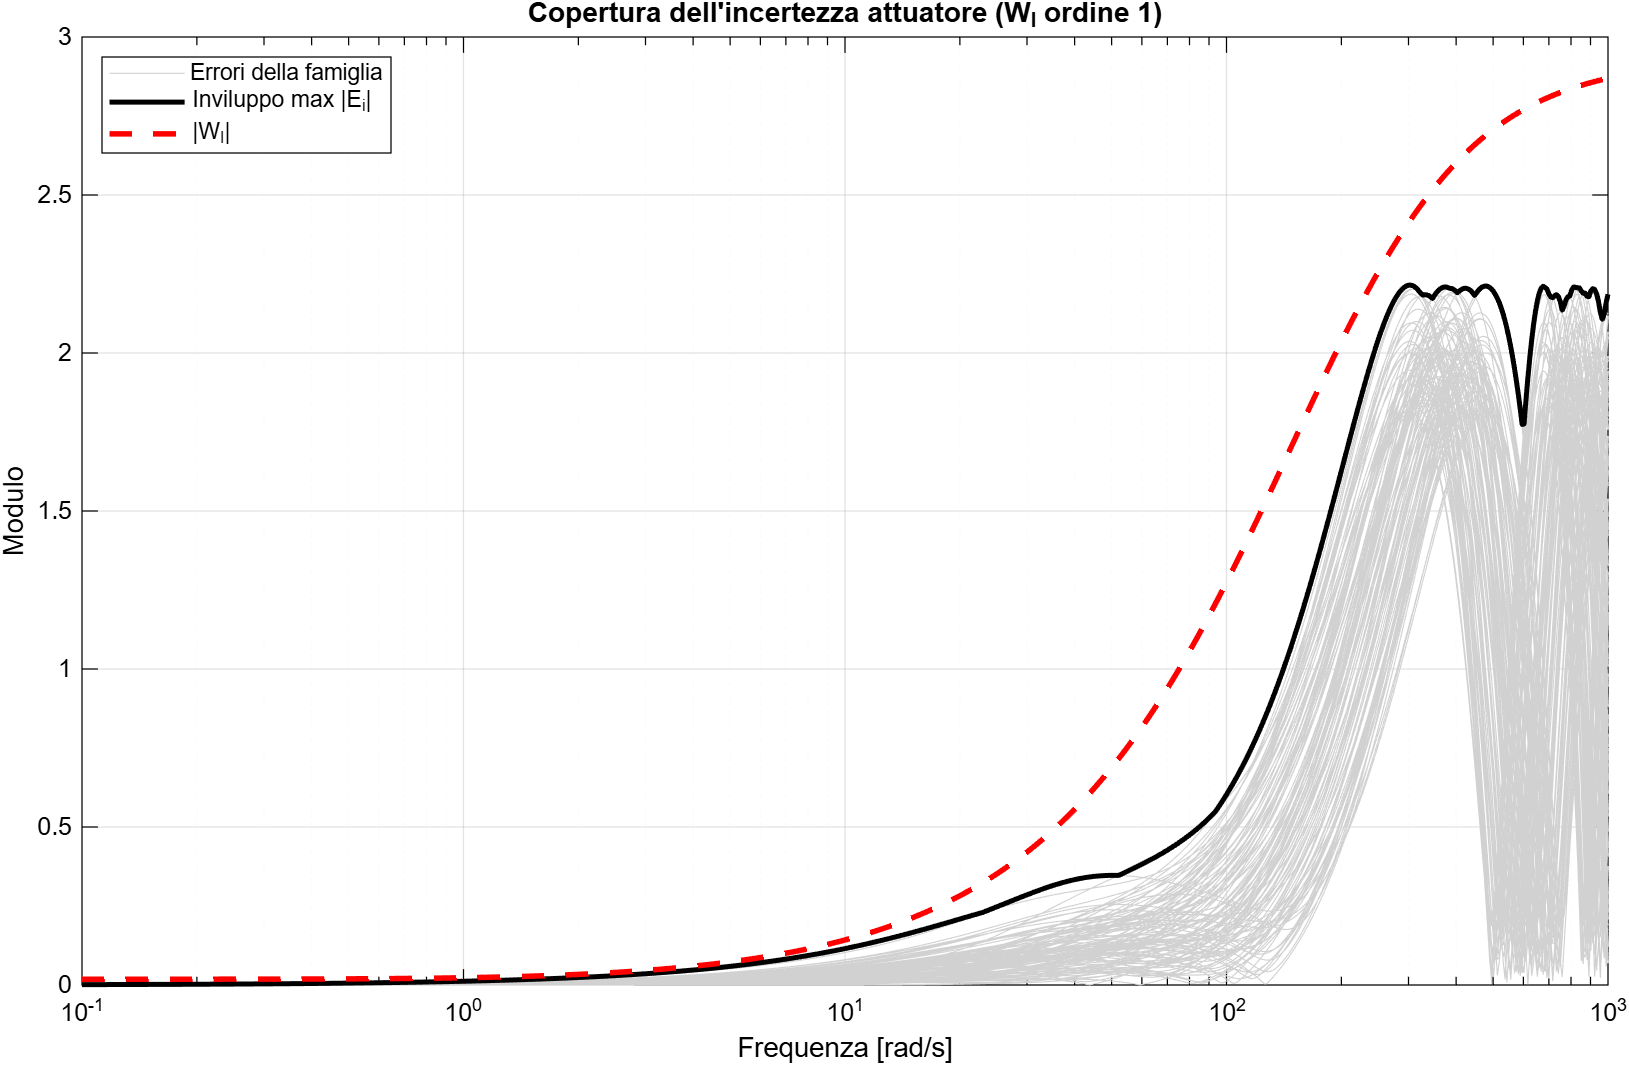
\includegraphics[width=0.78\textwidth]{figures/student_baseline/actuator_uncertainty.png}
\caption{Errore moltiplicativo della famiglia e copertura mediante $W_I$.}\label{fig:m4-wi}
\end{figure}


\medskip\noindent\textbf{Limite della copertura moltiplicativa con Pad\'e.}
La verifica in modulo sulla griglia non dimostra che l'errore normalizzato
sia una dinamica stabile. Con $T_0=0.015$ s, il nominale razionale
$G_{a0}=H_0P_{T_0}$ contiene
\[
 H_{\omega,\zeta}(s)=\frac{\omega^2}{s^2+2\zeta\omega s+\omega^2},
 \qquad P_T(s)=\frac{1-Ts/2}{1+Ts/2}.
\]
$P_{T_0}$ ha uno zero a $s=2/T_0=133.33$ rad/s nel semipiano destro.
Già per il ritardo esatto nominale, $e^{-T_0s}/P_{T_0}(s)-1$
ha un polo in quel punto, con residuo $-4e^{-2}/T_0\ne0$.
Poiché $W_I$ storico non cancella tale polo, la corrispondente
$\Delta$ non appartiene alla classe stabile di \texttt{ultidyn}.
I certificati storici restano validi per il loro modello matematico,
ma la sola copertura frequenziale non li trasferisce all'intera famiglia
con ritardo esatto. Il modello moltiplicativo e i relativi risultati sono
conservati senza ricalcolo o sostituzione degli archivi.

\medskip\noindent\textbf{Due rappresentazioni per lo stesso dominio fisico.}
Il confronto aggiuntivo mantiene $\omega\in[36,44]$ rad/s,
$\zeta\in[0.72,0.88]$ e $T\in[0.012,0.018]$ s, indipendenti per
ciascun attuatore. Sono ritardi costanti incerti; la certificazione non
include jitter arbitrariamente variabile nel tempo. Indichiamo gli estremi
con $\omega_\pm,\zeta_\pm,T_\pm$ e il nominale con il pedice zero.
La rappresentazione parametrica B è
\[
 G_{a,B}=H_{\omega,\zeta}(P_T+W_R\Delta_R),\qquad
 \|\Delta_R\|_\infty\le1,
 \qquad
 W_R=\kappa\left(\frac{T_+s}{1+T_+s}\right)^3,
 \quad \kappa=\frac{(1+24^{2/3})^{3/2}}{12}.
\]
Infatti, per $x=|\Omega T|$,
$|e^{-j\Omega T}-P_T(j\Omega)|\le\min(2,x^3/12)$:
la differenza di fase $x-2\arctan(x/2)$ è al più $x^3/12$.
Il massimo del rapporto tra questa maggiorazione e
$(x/\sqrt{1+x^2})^3$ è $\kappa$.
Il residuo normalizzato ha una singolarità rimovibile all'origine,
è stabile e limitato anche ad alta frequenza. Il residuo fisico dipende
da $T$; renderlo indipendente in B allarga l'insieme e introduce
conservatività dichiarata. Il nominale di B resta $H_0P_{T_0}$:
il ritardo esatto nominale è un altro membro della famiglia, con
$\Delta_R\ne0$.

La LFT manuale usa $x_a, v_a=\dot x_a$ per il secondo ordine e $h$ per
Pad\'e. Con $\omega=\omega_0(1+0.1\delta_\omega)$,
$\zeta=\zeta_0(1+0.1\delta_\zeta)$ e
$T=T_0(1+0.2\delta_T)$, apriamo le porte
\[
 \begin{aligned}
 a&=\omega_0(u-x_a+0.1w_{\omega1}),&
 b&=a-2\zeta_0(v_a+0.1w_\zeta),\\
 \dot v_a&=\omega_0(b+0.1w_{\omega2}),&
 \dot h&=2(x_a-h)/T_0-0.2w_T,\\
 y_P&=2h-x_a,& y_a&=y_P+W_Rw_R,
 \end{aligned}
\]
con $v_\Delta=[u-x_a,b,v_a,\dot h,x_a]^\top$ e
\[
 w_\Delta=\Delta_a v_\Delta,\qquad
 \Delta_a=\operatorname{diag}
 (\delta_\omega I_2,\delta_\zeta,\delta_T,\Delta_R).
\]
Le due occorrenze di $\delta_\omega$ sono lo stesso scalare, non due
incertezze indipendenti: richiudendole si ricostruiscono sia
$\omega^2$ sia $2\zeta\omega$. Il loop di $\delta_T$ produce
$1/T$ esattamente ed è ben posto, poiché $1+0.2\delta_T\ge0.8$.
La matrice nota attuativa è $6\times6$ e $\Delta_a$ è $5\times5$.
Con due attuatori e la meccanica, B ha nove scalari reali distinti e due
blocchi dinamici, con dimensione totale di $\Delta$ pari a 13.
\begin{center}
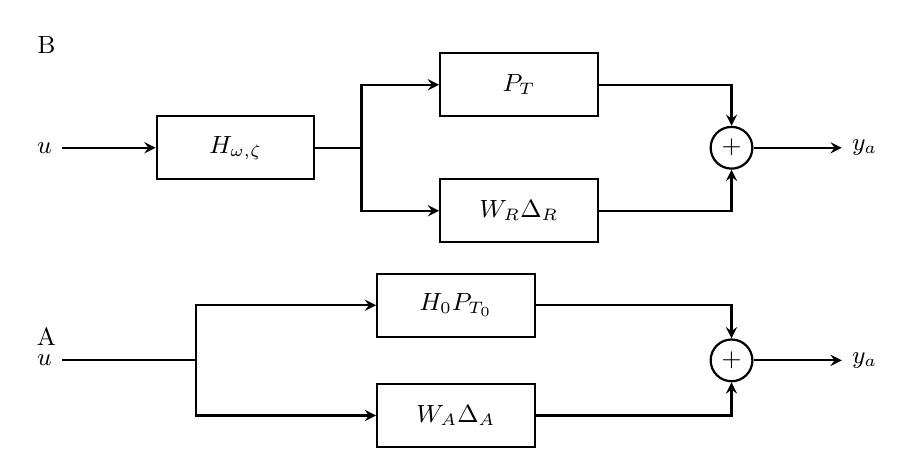
\begin{tikzpicture}[>=stealth,thick,every node/.style={font=\small},
 b/.style={draw,align=center,minimum width=2cm,minimum height=.8cm}]
\node at (-5.4,1.3) {B};
\node[b] (h) at (-3,0) {$H_{\omega,\zeta}$};
\node[b] (p) at (.6,.8) {$P_T$};
\node[b] (r) at (.6,-.8) {$W_R\Delta_R$};
\node[draw,circle,inner sep=2pt] (s) at (3.3,0) {$+$};
\draw[->] (-5.2,0) node[left] {$u$} -- (h);
\draw[->] (h.east) -- (-1.4,0) |- (p.west);
\draw[->] (-1.4,0) |- (r.west);
\draw[->] (p.east) -| (s.north);
\draw[->] (r.east) -| (s.south);
\draw[->] (s.east) -- (4.7,0) node[right] {$y_a$};
\node at (-5.4,-2.4) {A};
\node[b] (n) at (-.2,-2) {$H_0P_{T_0}$};
\node[b] (a) at (-.2,-3.4) {$W_A\Delta_A$};
\node[draw,circle,inner sep=2pt] (sa) at (3.3,-2.7) {$+$};
\draw[->] (-5.2,-2.7) node[left] {$u$} -- (-3.5,-2.7) |- (n.west);
\draw[->] (-3.5,-2.7) |- (a.west);
\draw[->] (n.east) -| (sa.north);
\draw[->] (a.east) -| (sa.south);
\draw[->] (sa.east) -- (4.7,-2.7) node[right] {$y_a$};
\end{tikzpicture}

\end{center}

La rappresentazione concentrata A raccoglie invece lo scarto additivo
rispetto allo stesso nominale:
\[
 G_{a,A}=H_0P_{T_0}+W_A\Delta_A,\qquad \|\Delta_A\|_\infty\le1.
\]
Per costruire il peso senza il polo spurio dell'inversione di Pad\'e,
definiamo $a=\max_{\omega\in[\omega_-,\omega_+]}|\omega^2-\omega_0^2|$
e $b=\max_{\omega,\zeta}|2\zeta_0\omega_0\omega^2-2\omega_0^2\zeta\omega|$.
Il codice valuta anche gli eventuali punti stazionari interni per $b$.
Usiamo le maggiorazioni stabili
\[
 \begin{aligned}
 W_H(s)&=\frac{\sqrt2\,s(as+b)}
 {\zeta_-(s+\omega_-)^2(s^2+2\zeta_0\omega_0s+\omega_0^2)},\\
 W_T(s)&=\frac{\max(T_+-T_0,T_0-T_-)s}
 {(1+T_-s/2)(1+T_0s/2)},\qquad
 \overline H(s)=\frac{\omega_+^2}{\zeta_-(s+\omega_-)^2}.
 \end{aligned}
\]
Per $0<\zeta_-\le1$ vale
$|(j\Omega)^2+2\zeta\omega j\Omega+\omega^2|
\ge\zeta_-(\omega^2+\Omega^2)$.
La differenza dei due secondi ordini dà quindi
$|H_{\omega,\zeta}-H_0|\le|W_H|$;
inoltre $|P_T-P_{T_0}|\le|W_T|$ e $|H_{\omega,\zeta}|\le|\overline H|$.
Il peso $W_A$ è il fattore spettrale stabile, con zeri nel semipiano
sinistro salvo quello all'origine, definito da
\[
 |W_A|^2=3\bigl(|W_H|^2+|H_0W_T|^2+|\overline H W_R|^2\bigr).
\]
La disuguaglianza $(a_1+a_2+a_3)^2\le3\sum a_i^2$ applicata a
$(H-H_0)P_T+H_0(P_T-P_{T_0})+HW_R\Delta_R$ dimostra
$|G_{a,B}-G_{a0}|\le|W_A|$. La normalizzazione additiva è stabile:
lo zero all'origine è rimovibile e il grado relativo due del peso
è compatibile con gli scarti attuativi. Ne segue
$\mathcal G_{\rm fisica}\subseteq\mathcal G_B\subseteq\mathcal G_A$
per il dominio unitario, senza postulare la stessa inclusione per ogni
scala dei margini robusti. A ha cinque blocchi totali, come numero ma
non come significato uguali al modello storico. Non costituisce una
nuova sintesi o un terzo progetto: serve a misurare la conservatività
della concentrazione rispetto alla rappresentazione parametrica.

\section{Verifica e limiti}
La struttura contiene \MFourBlockCount\ blocchi: tre \texttt{ureal} e due \texttt{ultidyn}. Il valore nominale delle viste verso $[q;\theta]$ e verso $q$ coincide con il modello completo entro $10^{-8}$. Quaranta campioni \texttt{usample} rispettano i range e producono sistemi finiti delle dimensioni attese.

Questa verifica riguarda la costruzione dell'ensemble, non la robustezza in anello chiuso. I range sono intervalli ammissibili, non densità di probabilità: per questo un campionamento uniforme usato nelle prove pratiche non autorizza un'interpretazione probabilistica dei conteggi. Le conclusioni RS/RP appartengono alla $\mu$-analysis. Anche il campionamento successivo resta evidenza empirica e non sostituisce la certificazione strutturata.

Le verifiche aggiuntive, separate dalla campagna storica, confrontano le due
LFT attuative con una realizzazione automatica indipendente su otto vertici
e 24 punti interni per canale, includendo un residuo dinamico stabile non
nullo. Lo scarto massimo è $1.45\cdot10^{-15}$; il fattore spettrale
soddisfa l'identità con errore relativo $1.05\cdot10^{-14}$ su 2401
frequenze. Nei campioni fisici i massimi rapporti residuo/$W_R$ e scarto/$W_A$
sono 0.885 e 0.339. Questi ultimi sono controlli numerici, mentre la
copertura continua discende dalle disuguaglianze precedenti. Il confronto
a controllore fissato è discusso nel Capitolo 9; non modifica $W_e,W_u,M_o$.
